\uuid{KE7m}
\exo7id{5552}
\auteur{rouget}
\organisation{exo7}
\datecreate{2010-07-15}
\isIndication{false}
\isCorrection{true}
\chapitre{Conique}
\sousChapitre{Parabole}

\contenu{
\texte{
Equation cartésienne de la parabole tangente à $(0x)$ en $(1,0)$ et à $(0y)$ en $(0,2)$.
}
\reponse{
On cherche l'équation d'une telle parabole $\mathcal{P}$ sous la 
forme $(ax+by)^2+2cx+2dy+e=0,\;a^2+b^2=1,\;a>0$.

$$(1,0)\in\mathcal{P}\Leftrightarrow\boxed{a^2+2c+e=0}\;\mbox{et}\;(0,2)\in\mathcal{P}\Leftrightarrow \boxed{4b^2+4d+e=0}.$$
D'après la règle de dédoublement des termes, une équation cartésienne de la tangente à
$\mathcal{P}$ en $(1,0)$ est $a^2x+aby+c(x+1)+dy+e=0$ ou encore $(a^2+c)x+(ab+d)y+c+e=0$. Cette tangente est l'axe
$(Ox)$ si et seulement si \shadowbox{$a^2+c=c+e=0\;\mbox{et}\;ab+d\neq0$.}
Une équation cartésienne de la tangente à
$\mathcal{P}$ en $(0,2)$ est $2abx+2b^2y+cx+d(y+2)+e=0$ ou encore $(2ab+c)x+(2b^2+d)y+2d+e=0$. Cette tangente est l'axe
$(Oy)$ si et seulement si \shadowbox{$2b^2+d=2d+e=0$\; et \;$2ab+c\neq0$.}
En résumé, $\mathcal{P}$ est solution si et seulement si

$$\left\{
\begin{array}{l}
c=-a^2\\
d=-2b^2\\
e=a^2=4b^2\\
a^2+b^2=1\\
ab+d\neq0\\
2ab+c\neq0\\
a>0
\end{array}
\right..$$
Maintenant, $\left(a^2=4b^2,\;a^2+b^2=1\;\mbox{et}\;a>0\right)\Leftrightarrow a=\frac{2}{\sqrt{5}}\;\mbox{et}\;b=\pm\frac{1}{\sqrt{5}}$. Le
cas $b=\frac{1}{\sqrt{5}}$ fournit $d=-\frac{2}{5}$ puis $ab+d=0$ ce qui est exclu. Donc, nécessairement
$a=\frac{2}{\sqrt{5}}$ et $b=-\frac{1}{\sqrt{5}}$ puis $c=-\frac{4}{5}$, $d=-\frac{2}{5}$ et $e=\frac{4}{5}$ qui 
sont effectivement solution du système.
On obtient ainsi une et une seule courbe du second degré solution, à savoir la courbe d'équation cartésienne

\begin{center}
\shadowbox{
$(2x-y)^2-8x-4y+4=0.$
}
\end{center}
Il reste à vérifier que cette courbe est effectivement une parabole.
On pose $\left\{
\begin{array}{l}
X=\frac{1}{\sqrt{5}}(-x-2y)\\
Y=\frac{1}{\sqrt{5}}(2x-y)
\end{array}
\right.$ ou encore $\left\{
\begin{array}{l}
x=\frac{1}{\sqrt{5}}(-X+2Y)\\
y=\frac{1}{\sqrt{5}}(-2X-Y)
\end{array}
\right.$.

\begin{align*}\ensuremath
(2x-y)^2-8x-4y+4=0&\Leftrightarrow5Y^2-\frac{8}{\sqrt{5}}(-X+2Y)-\frac{4}{\sqrt{5}}(-2X-Y)+4=0\Leftrightarrow5Y^2-\frac{12}{\sqrt{5}}Y+\frac{16}{\sqrt{5}}X+4=0\\
 &\Leftrightarrow5\left(Y-\frac{6}{5\sqrt{5}}\right)^2=-\frac{16}{\sqrt{5}}\left(X+\frac{4}{5\sqrt{5}}\right).
\end{align*}
$\mathcal{C}$ est donc effectivement une parabole.

$$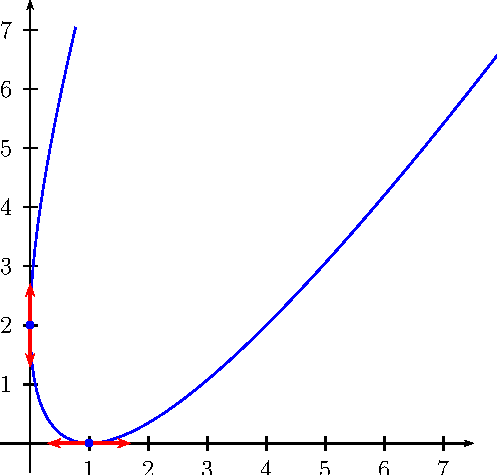
\includegraphics{../images/img005552-1}$$
}
}
